\chapter{Evaluación de la calidad en imágenes de fondo de ojo}


\section{Necesidad de un método automático de evaluación de calidad}
La calidad de una imagen de fondo de ojo se considera adecuada cuando permite visualizar claramente las estructuras patológicas relevantes. En el caso de un ojo sano, estas estructuras incluyen el disco óptico, la mácula y los vasos sanguíneos. Sin embargo, diversos factores, como el desenfoque, artefactos de iluminación, obstrucciones, niebla, suciedad en las lentes o la cámara, y distorsiones causadas por la refracción de la luz, pueden degradar la calidad de estas imágenes. A pesar de eso, en términos prácticos, la calidad de una imagen se define por su utilidad para el diagnóstico clínico. Esto significa que, en ciertos casos, una imagen con artefactos\footnote{Artefactos: Distorsiones o errores visuales no deseados en una imagen, que pueden originarse por fallos en el proceso de captura, compresión o procesamiento, y que no están presentes en la escena original.
} puede ser considerada de buena calidad si permite al oftalmólogo realizar una evaluación precisa.

El creciente volumen de datos en el campo de la salud visual ha hecho evidente que la evaluación subjetiva de la calidad, tradicionalmente realizada por expertos, resulta poco práctica y propensa a inconsistencias. Esto ha impulsado la búsqueda de métodos objetivos y automatizados que puedan replicar el juicio clínico humano con alta precisión, eliminando la carga operativa que supone la revisión manual.

Actualmente, existen muchos algoritmos diseñados para clasificar imágenes, pero la mayoría se han desarrollado utilizando imágenes naturales como referencia. Estas imágenes poseen propiedades estadísticas específicas, conocidas como "valores de naturalidad", que describen la distribución de características visuales como la intensidad de colores, el contraste, el brillo y las texturas. En imágenes naturales, se ha observado que la combinación de estas propiedades puede ser modelada utilizando una distribución Gaussiana multivariante. Sin embargo, las imágenes de fondo de ojo presentan propiedades distintas, lo que hace que sus valores de naturalidad no sigan este patrón. Como resultado, los algoritmos entrenados con imágenes naturales no suelen ser adecuados para evaluar la calidad de imágenes oftalmológicas. Además, la calidad de una imagen de fondo de ojo puede depender del tipo de diagnóstico que se realice. Por ejemplo, una imagen con regiones oscuras puede ser adecuada para la evaluación de glaucoma, pero inadecuada para el diagnóstico de retinopatía diabética \parencites{giancardo2010}. Esto subraya la necesidad de desarrollar soluciones específicas para este ámbito, capaces de analizar de manera robusta y eficiente la calidad de estas imágenes \parencites{piyasena2018}.

\section{Métodos basados en el diseño manual de características}
Los primeros modelos de evaluación de calidad de imágenes de fondos de ojo se desarrollaron a partir de medidas de similitud. A partir de imágenes de referencia de buena calidad, se calculaban atributos, como la distribución de la intensidad, que luego se comparaban con la de las nuevas imágenes. El inconveniente de esta metodología era que el histograma es una medida global de la imagen y no considera la ubicación de los píxeles. Por lo tanto, dos imágenes distintas podrían tener el mismo histograma, y, en algunos casos, una podría ser de buena calidad y la otra no (como se muestra en la Figura \ref{fig:Histograma_Intensidades} y Figura \ref{fig:retina_del_histograma}). Una mejora en este sentido fue la comparación local de los atributos, dividiendo la imagen en subregiones. Sin embargo, estas primeras soluciones tienen ciertas limitaciones a la hora de generalizarlas, dado que es imposible obtener un conjunto de atributos que sirva para todos los casos. Además, son algoritmos sensibles a las distorsiones que pueden presentar las imágenes y, al no considerar las diferentes estructuras del ojo, no reflejan completamente el criterio de los oftalmólogos.

\begin{center}
	\begin{figure}[H]
		\centering
		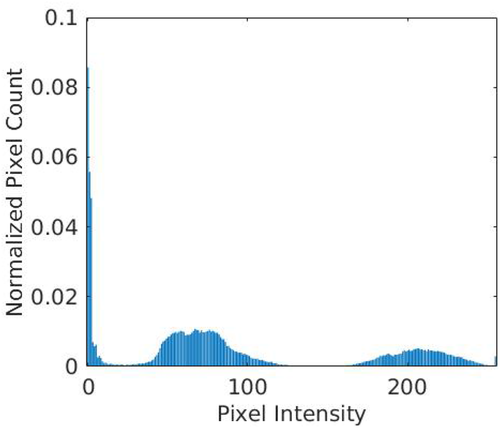
\includegraphics[scale=0.80]{doc_images/histograma_intensidad.png}
		\caption{Histograma normalizado de ambas imágenes de fondo de ojo. Fuente: \parencite{piyasena2018}.} 
		\label{fig:Histograma_Intensidades}
	\end{figure}
\end{center}

\begin{center}
	\begin{figure}[H]
		\centering
		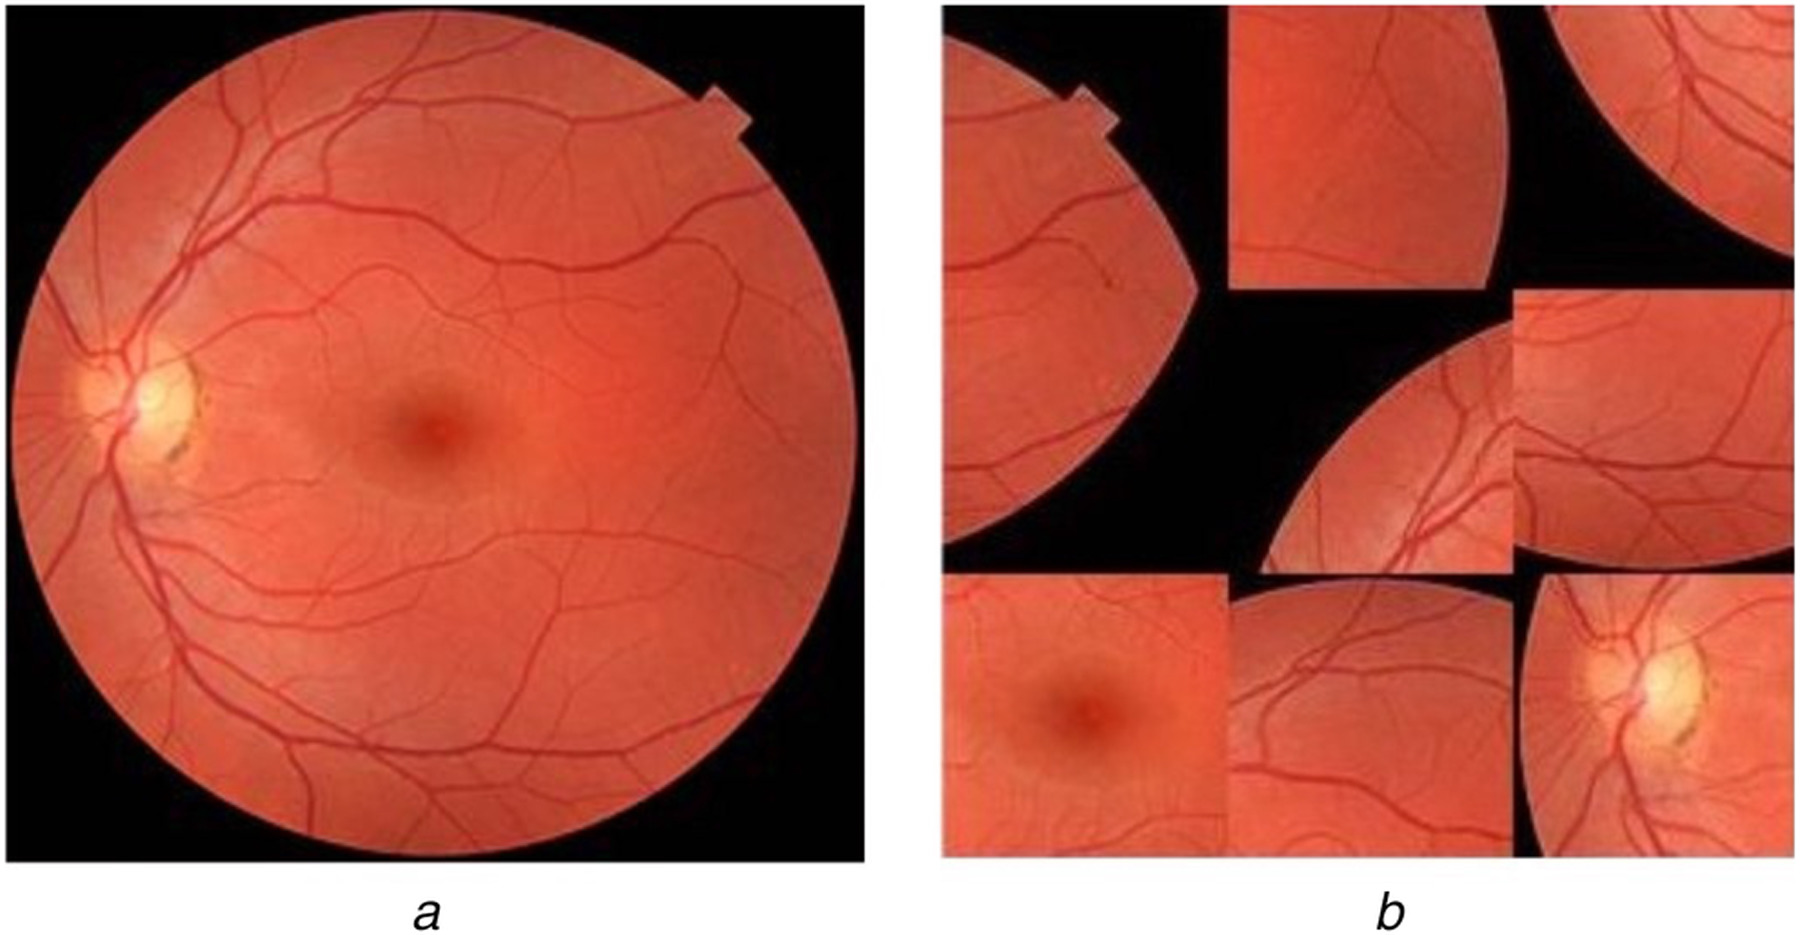
\includegraphics[scale=0.30]{doc_images/retina_del_histograma.jpg}
		\caption{Imágenes de fondo de ojo. (a) Buena calidad, (b) Mala calidad. Fuente: \parencite{piyasena2018}.} 
		\label{fig:retina_del_histograma}
	\end{figure}
\end{center}

Otros modelos se basaron en métodos de segmentación para detectar las diferentes estructuras del ojo (Figura \ref{fig:macula_do_vasos}). Inicialmente, la cantidad de píxeles asociados a los vasos sanguíneos se utilizaba como indicador de calidad, asumiendo que una mayor cantidad indicaba una mejor calidad. Posteriormente, se introdujeron mejoras, como el análisis de los vasos sanguíneos alrededor de la mácula, estructuras pequeñas y estrechas que son especialmente susceptibles a distorsiones y, por tanto, útiles como medida de calidad. También se incorporó la evaluación de la posición absoluta de la fóvea\footnote{Fóvea: Pequeña depresión en el centro de la mácula responsable de la visión aguda y detallada.} y la distancia promedio de los vasos respecto a esta. Finalmente, para abordar el problema del desenfoque, se utilizó el contraste entre los vasos sanguíneos y el fondo como indicador principal de nitidez. Aunque estos algoritmos reflejan con mayor precisión el enfoque utilizado por los oftalmólogos para evaluar la calidad de las imágenes, también presentan ciertos inconvenientes al intentar generalizarlos. Por un lado, operan bajo supuestos fijos sobre la forma, tamaño y posición de las estructuras del ojo, lo que puede limitar su desempeño al analizar imágenes que no se ajusten a esas características. Por otro lado, aunque incluyen el manejo de ruido, como el desenfoque, suelen estar diseñados para tratar tipos específicos de ruido, lo que significa que podrían fallar al enfrentarse a ruidos distintos de los previstos durante su desarrollo.

\begin{center}
	\begin{figure}[ht]
		\centering
		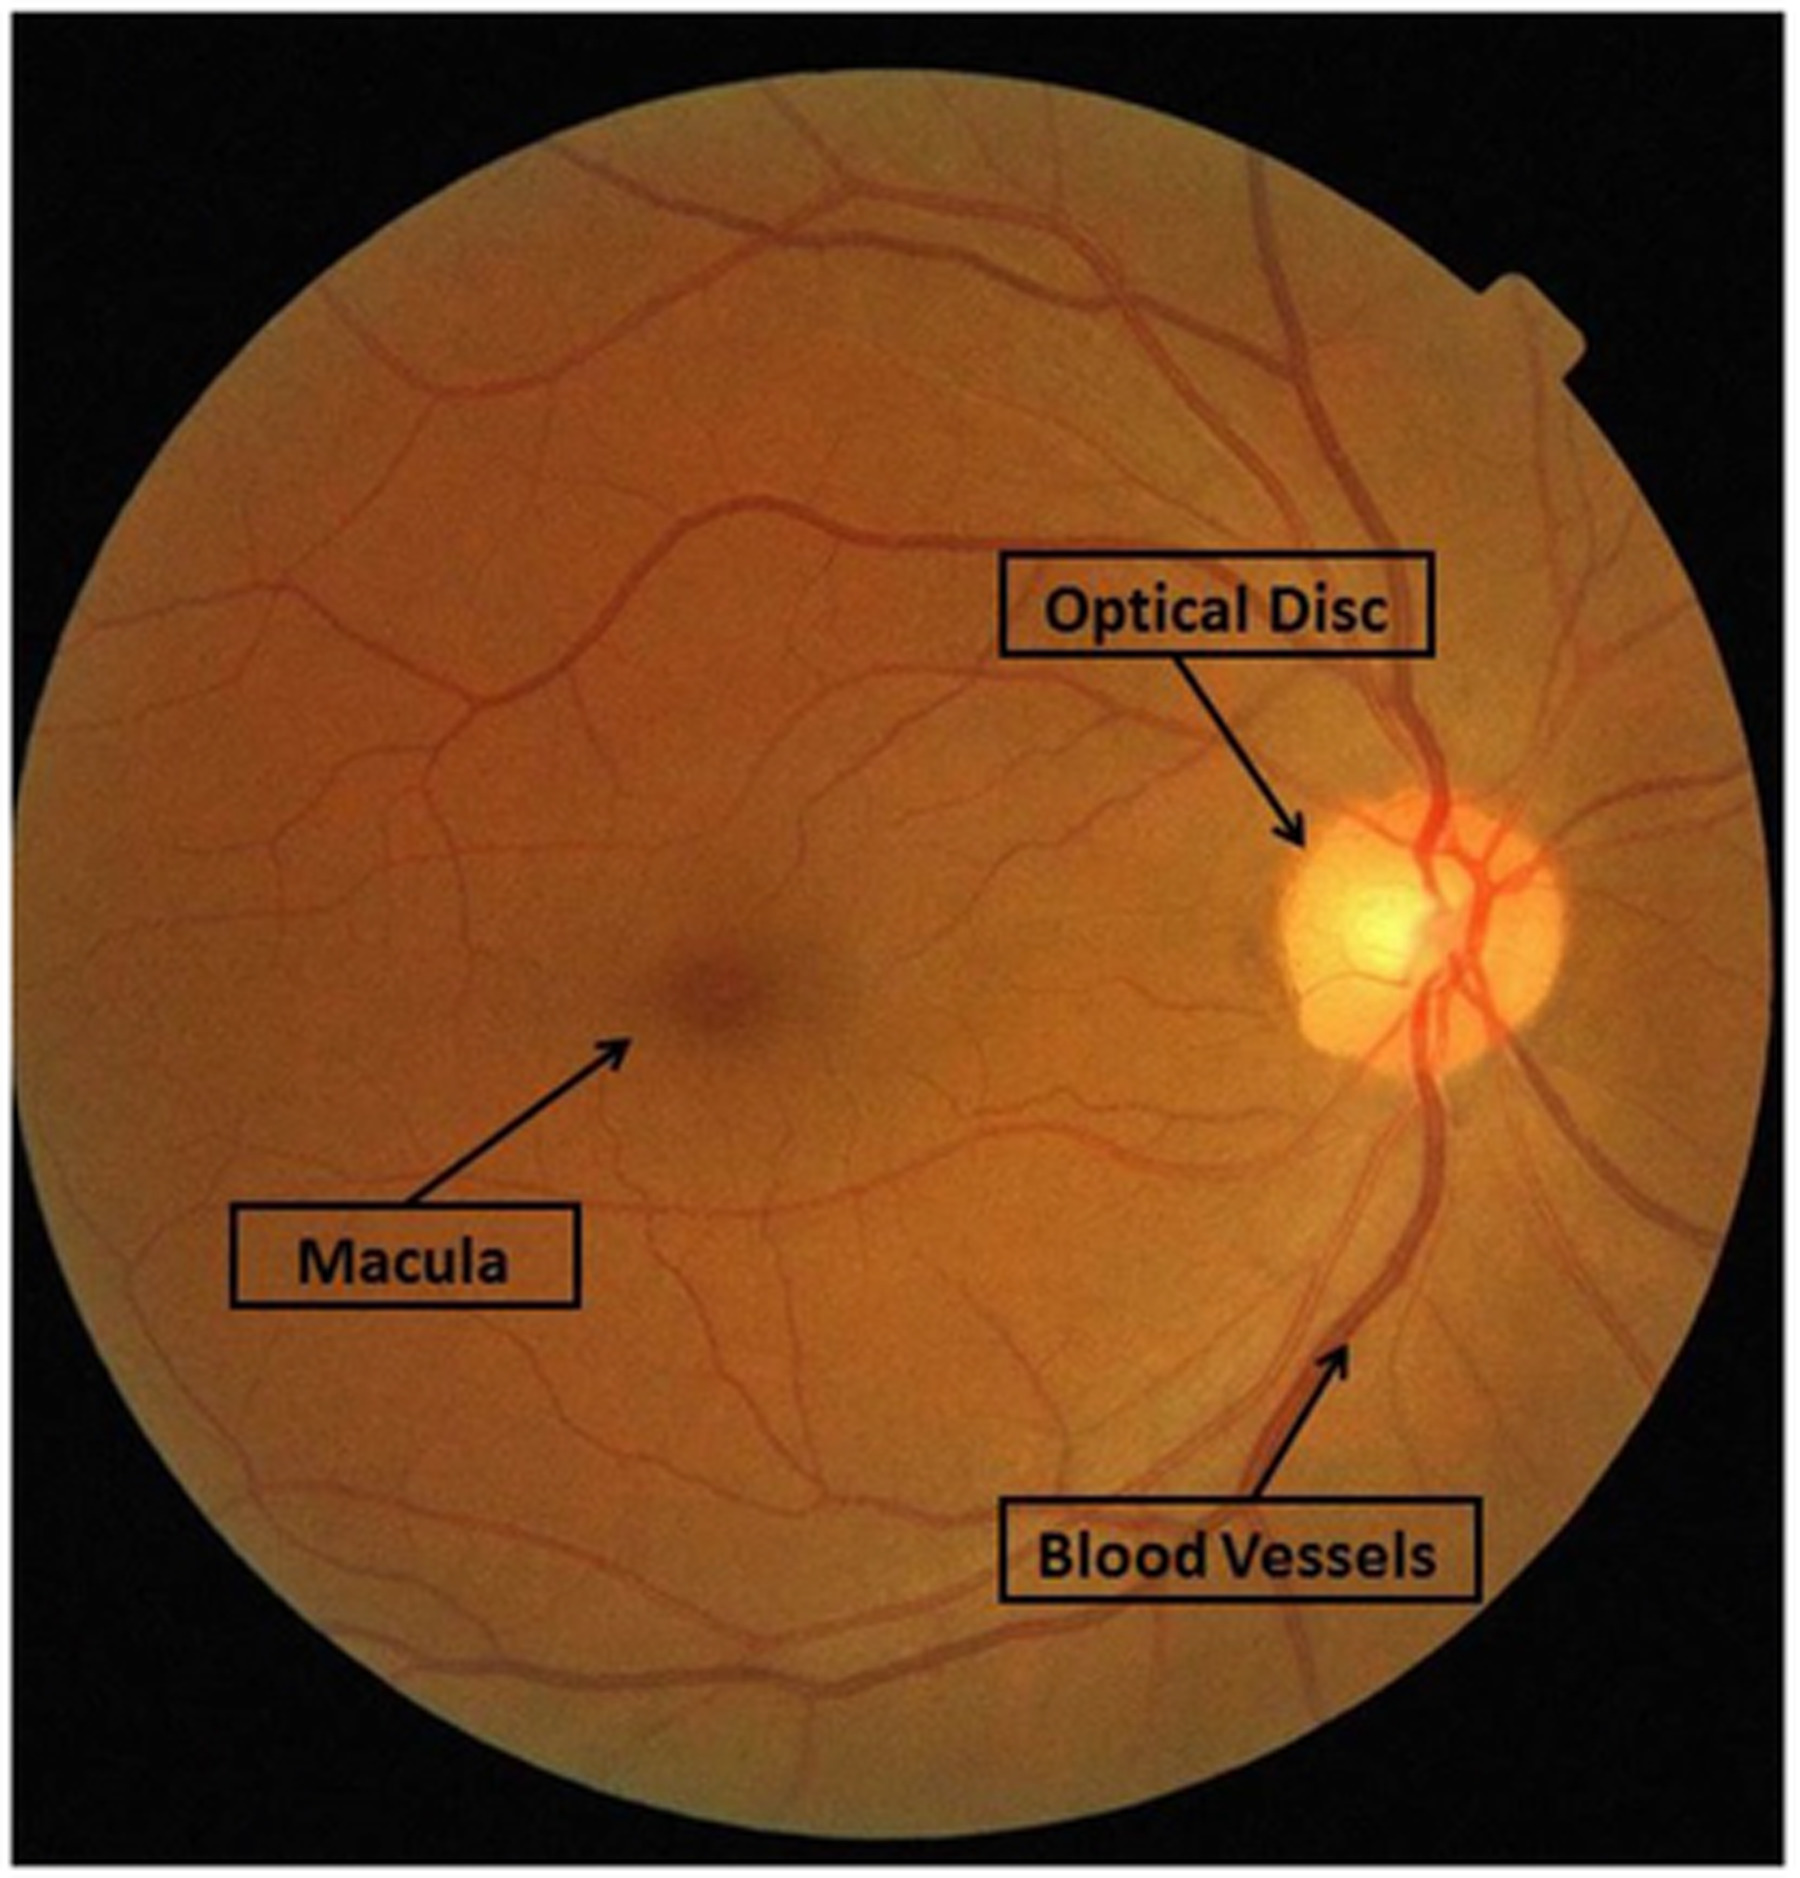
\includegraphics[scale=0.15]{doc_images/macula_do_vasos.jpg}
		\caption{Imagen de fondo de ojo donde se pueden observar las estructuras principales: mácula, disco óptico y vasos sanguíneos. Fuente: \parencite{piyasena2018}.} 
		\label{fig:macula_do_vasos}
	\end{figure}
\end{center}

Tanto las medidas de similitud como los métodos de segmentación fueron luego combinados y refinados para ser utilizados como predictores para entrenar diferentes algoritmos de machine learning, como SVM, regresión o k-NN, con el fin de realizar una clasificación binaria, multiclase o asignar un puntaje de calidad \parencite{piyasena2018}.
Los métodos basados en atributos hechos a mano dependen en gran medida del diseño de características, siendo demasiado complejo lograr características eficientes y apropiadas que se adapten a las variaciones y complejidades inherentes a las imágenes oftalmológicas \parencite{xu2020}. Esto genera limitaciones en el rendimiento, especialmente en condiciones no previstas o en imágenes con artefactos y ruidos inesperados.

\section{Métodos basados en la extracción automática de características}
Los métodos basados en redes neuronales han emergido como una solución innovadora para superar las limitaciones inherentes a los enfoques tradicionales en la evaluación de la calidad de imágenes de fondo de ojo. A diferencia de los métodos que dependen del diseño manual de características, las redes neuronales tienen la capacidad de aprender representaciones directamente a partir de los datos, eliminando la necesidad de intervención manual en la extracción de atributos. Esto es particularmente relevante, dado que la selección de características en los enfoques tradicionales es un proceso complejo, sujeto a sesgos y, a menudo, incapaz de capturar la diversidad de variaciones presentes en las imágenes clínicas. Las redes neuronales no solo automatizan este proceso, sino que también permiten identificar patrones complejos que los métodos tradicionales no pueden capturar. Además, logran distinguir entre características relevantes y artefactos irrelevantes, mejorando tanto la precisión como la robustez frente a variaciones en las condiciones de captura, como el desenfoque o los niveles de iluminación.

En 2016, \cite{mahapatra2016} propusieron el primer algoritmo basado en CNN para evaluar la calidad de imágenes de fondo de ojo. Sin embargo, se enfrentaron a dos desafíos: la escasa cantidad de imágenes para el entrenamiento (solo 101) y la falta de imágenes de mala calidad. Para superar estos problemas, extrajeron parches de 150×150 píxeles de las imágenes, etiquetándolos igual que las imágenes originales. Además, simularon distorsiones, como el ruido gaussiano, para generar imágenes de baja calidad que complementaran su conjunto de datos. De manera similar, \cite{costa2017eyequal} emplearon la técnica de dividir las imágenes en subregiones para clasificar cada una por separado y luego ponderar los resultados, obteniendo una clasificación final para la imagen completa.

El principal inconveniente de ambos enfoques es el tamaño reducido de la muestra, lo que dificulta el entrenamiento efectivo de una red neuronal. Para abordar este problema, \cite{yu2017image} utilizaron una CNN para extraer características, pero no para realizar la clasificación directamente. En su lugar, combinaron las salidas de la CNN con características manualmente construidas y utilizaron un SVM para clasificar las imágenes como de buena o mala calidad.

Uno de los principales desafíos al utilizar redes neuronales es la necesidad de grandes cantidades de datos etiquetados, lo cual es costoso y laborioso de obtener. Por esta razón, en los últimos años se ha explorado el uso de redes preentrenadas como una posible solución. Al aprovechar modelos previamente entrenados en grandes bases de datos, incluso si son imágenes naturales, los investigadores pueden realizar un fine-tuning para adaptarlos a tareas específicas, como la clasificación de calidad de imágenes retinianas. En este sentido, \cite{saha2018automated} utilizan la arquitectura AlexNet, inicializada con pesos preentrenados del modelo de referencia de Caffe\footnote{Caffe: Convolutional Architecture for Fast Feature Embedding, es un marco de aprendizaje profundo que admite una variedad de arquitecturas de aprendizaje profundo e incluye modelos preentrenados.} (entrenado en ImageNet\footnote{ImageNet:  Base de datos extensa con más de 14 millones de imágenes etiquetadas, utilizada ampliamente en la investigación de modelos de reconocimiento de objetos y entrenamiento de redes neuronales.}) y después realizan un fine-tuning para la evaluación de calidad de las retinografías. La arquitectura AlexNet consta de cinco capas convolucionales: la primera tiene 96 filtros de 11x11, la segunda 256 filtros de 5x5, la tercera y cuarta 384 filtros de 3x3, y la última 256 filtros de 3x3. Posteriormente, la red incluye dos capas completamente conectadas de 4096 neuronas cada una, seguidas de una capa completamente conectada de 1000 neuronas.  \cite{saha2018automated} reemplazan esta última capa por un clasificador binario para adaptar la red a su problema específico.

\begin{center}
	\begin{figure}[h]
		\centering
		
\includegraphics[scale=0.15]{doc_images/AlexNet_Original_block_diagram.svg.png}
		\caption{Arquitectura de la red neural convolucional AlexNet. Fuente: \parencites{krizhevsky2012imagenet}.} 
		\label{fig:AlexNet_Original_block_diagram}
	\end{figure}
\end{center}

En una línea similar, \cite{zago2018retinal} aplican la técnica de fine-tuning en una CNN VGG-16, una red más profunda con 16 capas en lugar de 8, que utiliza filtros más pequeños. Además, emplean distintos conjuntos de datos para el entrenamiento y la validación. De esta forma, haciendo validación cruzada dentro de cada conjunto y entre diferentes datasets, permite evaluar la capacidad del modelo para generalizar a datos provenientes de diversas fuentes.

\begin{center}
	\begin{figure}[H]
		\centering
		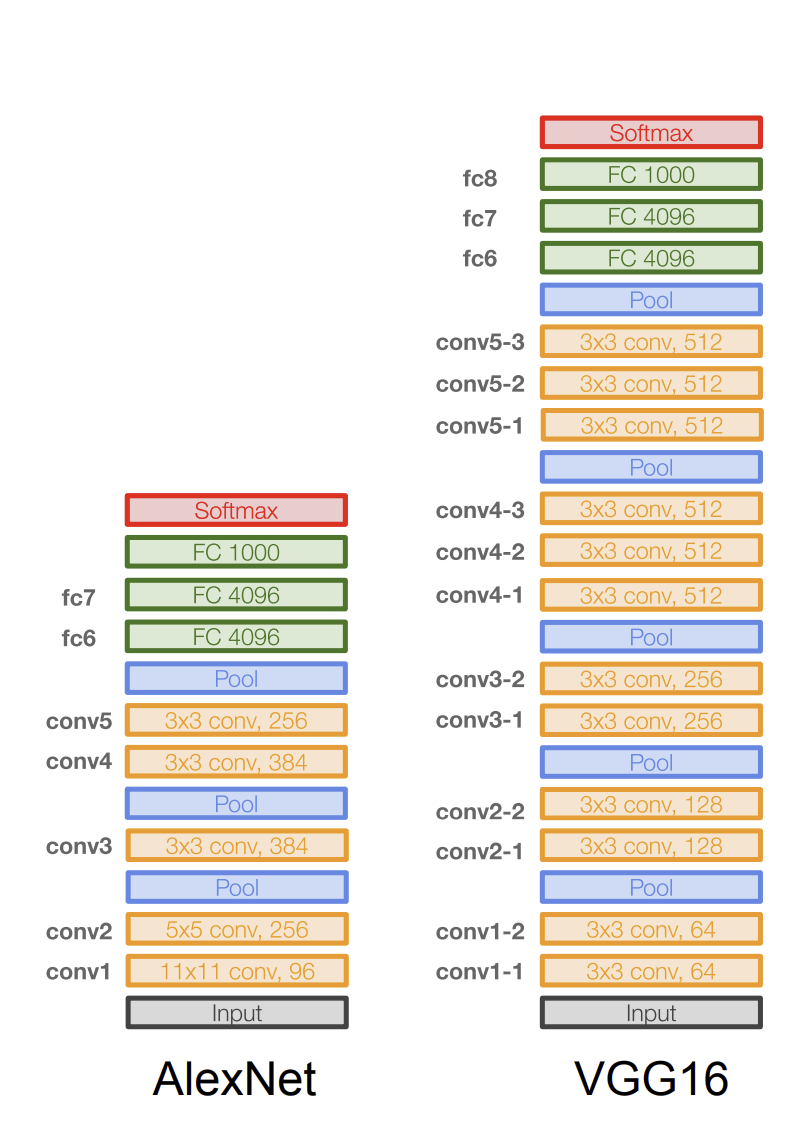
\includegraphics[scale=0.80]{doc_images/AlexNet_VGG16.png}
		\caption{Comparación entre arquitecturas de redes AlexNet y VGG16. Extraído de Convolutional Neural Networks for Visual Recognition [Diapositivas del curso], por K. Li, A. Karpathy, y J. Johnson, 2020, Universidad de Stanford, \url{https://cs231n.stanford.edu/slides/2020/lecture_9.pdf}.} 
		\label{fig:AlexNet_VGG16}
	\end{figure}
\end{center}

\cite{fu2019evaluation} analizan la influencia de los distintos espacios de color en la evaluación de calidad de imágenes retinianas, proponiendo una arquitectura llamada Multiple Color-space Fusion Network (MCF-Net). Esta red consta de dos bloques: un bloque base donde entrenan tres CNN en paralelo para cada uno de los espacios de color (RGB, HVS, LAB), generando un mapa de características para cada uno, y un segundo bloque donde fusionan la salida de las tres redes en una sola representación. Esta fusión de los tres canales junto con cada una de las representaciones individuales se utilizan como entrada para realizar la clasificación final. \cite{fu2019evaluation} demuestran que el rendimiento es superior cuando se consideran múltiples canales de color en comparación con el rendimiento de cada canal individualmente.

\begin{center}
	\begin{figure}[H]
		\centering
		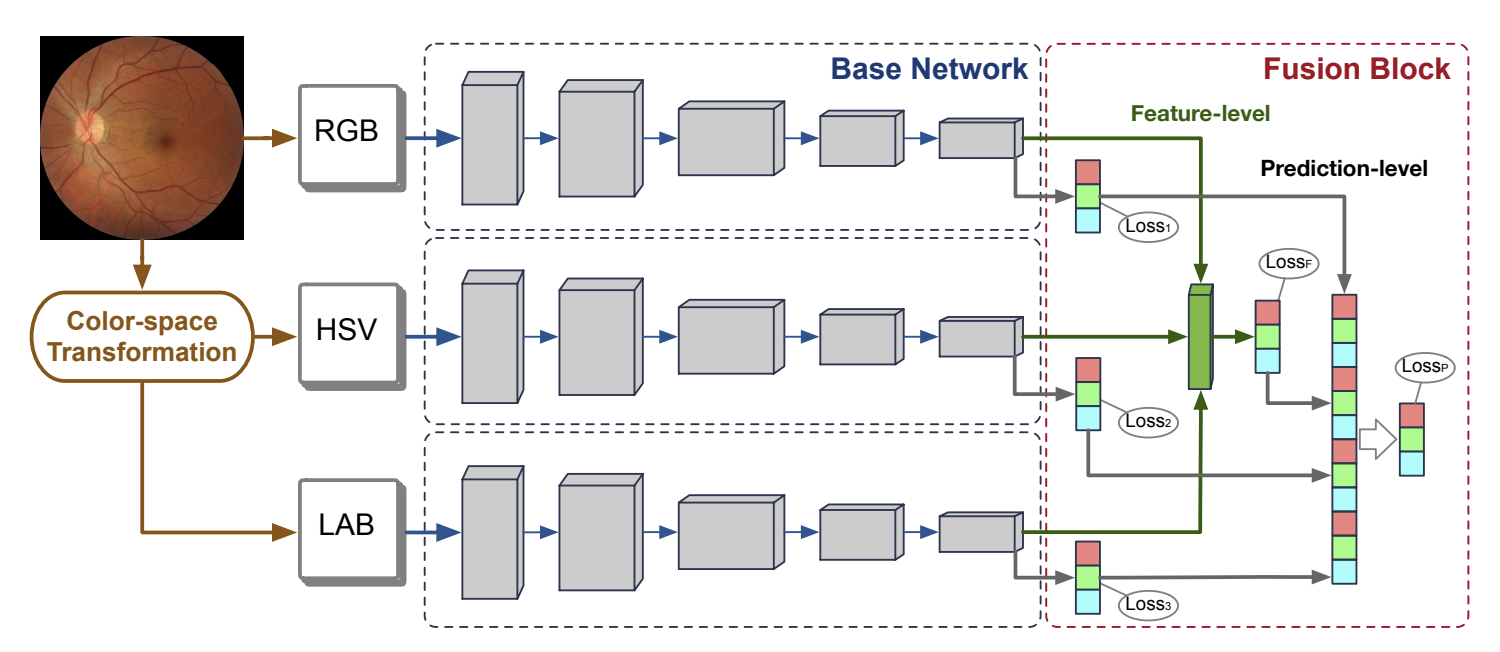
\includegraphics[scale=0.80]{doc_images/FU.png}
		\caption{Arquitectura MCF-Net \parencites{fu2019evaluation}.} 
		\label{fig:FU}
	\end{figure}
\end{center}

En este contexto, \cite{shen2018multi} afirman que las tareas auxiliares contribuyen a la evaluación de la calidad de las imágenes retinianas y proponen un marco de trabajo multi-tarea denominado Multi-task Fundus Image Quality Assessment (MFIQA).En este marco, una ResNet50, una red neuronal profunda que utiliza conexiones residuales para facilitar el entrenamiento de redes con muchas capas, se entrena para la detección del disco óptico y la mácula, mientras que una VGG16 se emplea para refinar la localización de estas estructuras. Además, se utilizan dos codificadores: uno para codificar imágenes retinianas completas en un sistema de coordenadas cartesianas, y otro para codificar ventanas locales del disco óptico en un sistema de coordenadas polares para la clasificación de la calidad de las imágenes. El modelo es entrenado para tres tareas auxiliares de clasificación de artefactos, claridad y definición de campo, que ayudan en el aprendizaje de la evaluación de calidad.

\begin{center}
	\begin{figure}[H]
		\centering
		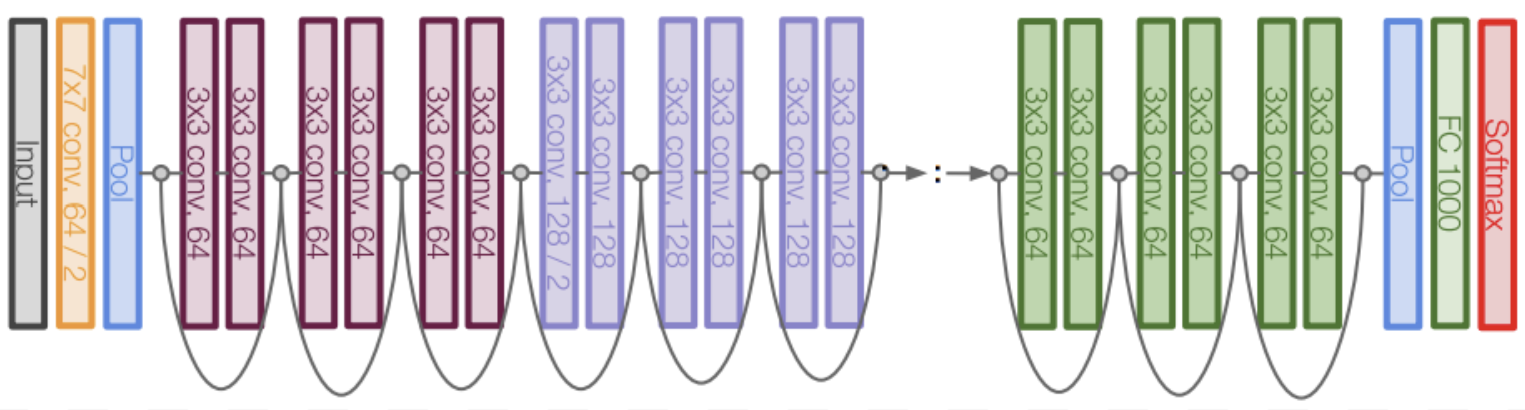
\includegraphics[scale=0.80]{doc_images/resnet.png}
		\caption{Arquitectura de redes residuales (ResNet) que puede tener 18, 34, 50, 101 o 152 capas. Extraído de Convolutional Neural Networks for Visual Recognition [Diapositivas del curso], por K. Li, A. Karpathy, y J. Johnson, 2020, Universidad de Stanford, \url{https://cs231n.stanford.edu/slides/2020/lecture_9.pdf}.} 
		\label{fig:resnet}
	\end{figure}
\end{center}

Tanto MCF-Net como MFIQA agregan características ricas que mejoran la clasificación, aunque en ambas arquitecturas, los parámetros a optimizar aumentan considerablemente. Además, el aprendizaje de tareas auxiliares requiere más anotaciones sobre las imágenes, lo cual resulta costoso \parencites{xu2020deep}. En este contexto, \cite{xu2020deep} retoman los fundamentos al destacar los elementos que los oftalmólogos consideran esenciales en una retinografía para evaluar su calidad. Su enfoque se centra en la detección de estructuras relevantes, diferenciando entre aquellas de pequeño tamaño, como los vasos sanguíneos, y las de mayor tamaño, como la mácula o el disco óptico. Estas estructuras se combinan con la imagen original para servir como entrada en el aprendizaje profundo de características y la posterior clasificación de calidad. Para incorporar estos priors\footnote{Priors: Información previa que se incorpora al modelo para guiar el proceso de aprendizaje.} de estructuras relevantes, proponen el modelo SalStructIQA (Salient Structure Image Quality Assessment), que tiene dos variantes: una de rama única y otra de dos ramas. En la primera, se concatenan la imagen original y los mapas de características de las estructuras pequeñas y grandes antes de proceder al aprendizaje profundo para la clasificación de calidad. En la variante de dos ramas, se utilizan dos CNN paralelas que aprenden separadamente las características de la imagen retiniana con estructuras grandes y pequeñas, fusionando posteriormente estas características para la evaluación de calidad.

\begin{center}
	\begin{figure}[H]
		\centering
		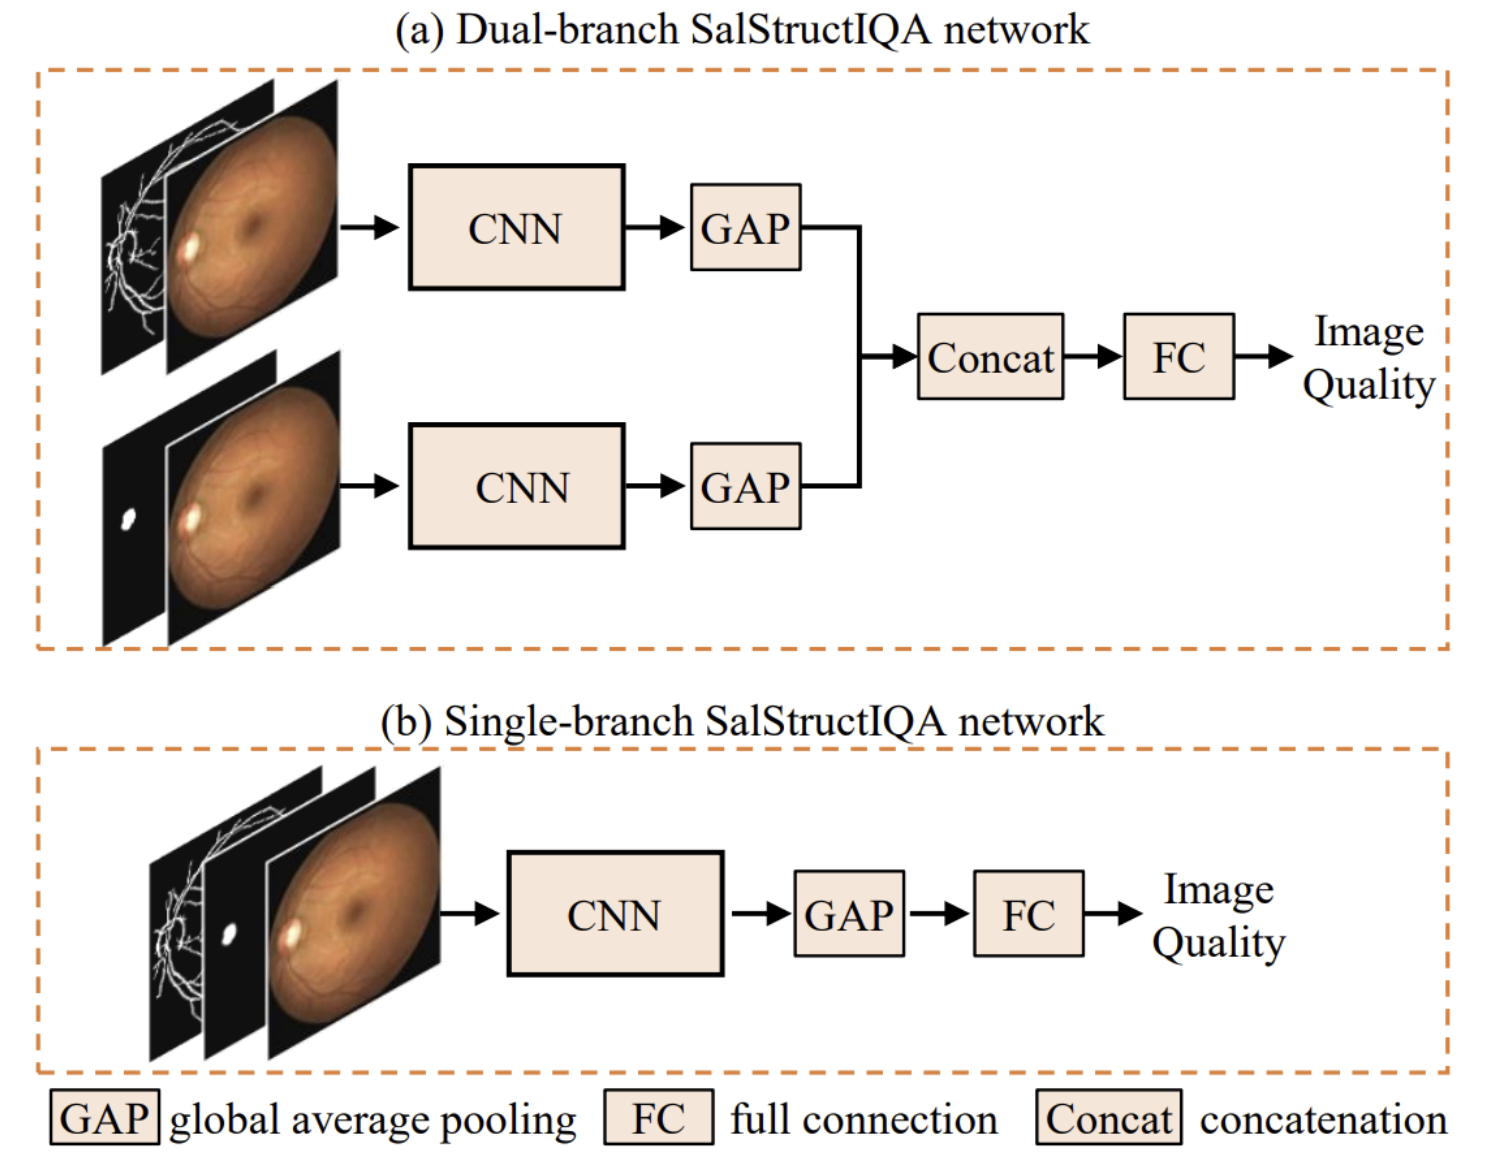
\includegraphics[scale=0.80]{doc_images/SalStructl.png}
		\caption{Dos implementaciones de la arquitectura SalStructlQA, \parencites{xu2020deep}.} 
		\label{fig:SalStructl}
	\end{figure}
\end{center}

En el cuadro \ref{tab:metodosQA}, que se encuentra en el anexo, se detallan los métodos de evaluación de calidad de imágenes de fondo de ojo.

